% --- repeat the title (AT: haven't found a more elegant way to do this...)
{
\vspace{2.0em}
\centering
\Large
\textbf{\blendfields: Few-Shot Example-Driven Facial Modeling} \\
\vspace{0.5em}
 Supplementary Material \\ \vspace{1.0em} }

 \section{Potential social impact} Our motivation for this work was to enable
 the creation of 3D avatars that could be used as communication devices in the
 remote working era.
  As our approach stems from blendshapes~\cite{lewis2014practice}, these
  avatars are easily adjustable via texture coloring and may be used for
  entertainment.
  We note, however, that the potential misuse of our work includes using it as
  deep fakes.
  We highly discourage such usage.
  One of our future directions includes detecting fake images generated by our
  method.
  At the same time, we highlight the importance of \blendfields---in the
  presence of closed technologies~\cite{ma2021pixel,cao2022authentic}, it is
  crucial to democratize techniques for personalized avatar creation.
  We achieve that by limiting the required data volume to train a single
  model.
  As history shows, when given an open, readily available technology for
  generative modeling of images~\cite{rombach2022high}, users can scrutinize
  it with unprecedented thoroughness, thus raising the general awareness of
  potential misuses.

\section{Concurrent Works}
  Gao~\etal~\cite{gao2022reconstructing} and Xu~\etal~\cite{xu2023avatarmav}
  also use an interpolation between known expressions to combine multiple
  neural radiance fields trained for those expressions.
  However, their approach interpolates between grids of latent
  vectors~\cite{mueller2022instant} globally.
  The interpolation weights are taken from blendshape coefficients.

  Zielonka~\etal~\cite{zielonka2022instant} use a parametric head model to
  canonicalize 3D points similarly to our ends.
  However, instead of building a tetrahedral cage around the head, they
  smoothly assign each face triangle to 3D points.
  Then they canonicalize points using transformations that each of the
  assigned triangles undergoes for a given expression.
  They concatenate 3D points with the expression code from
  FLAME~\cite{li2017flame} to model expression-dependent effects.

  \begin{table}[!t]
  \centering
  \resizebox{\linewidth}{!}{
    \begin{tabular}{ccccccc}
      \toprule
      \multirow{2}[2]{*}{\# expr.} & \multicolumn{3}{c}{Casual Expressions} & \multicolumn{3}{c}{Novel Pose Synthesis}                                                                                                                                                  \\
      \cmidrule{2-7}
                                   & PSNR $\uparrow$                        & SSIM $\uparrow$                          & LPIPS $\downarrow$                & PSNR $\uparrow$                    & SSIM $\uparrow$                   & LPIPS $\downarrow$                \\
      \midrule
      $\nExpr{=}1$                 & 27.5834                                & 0.9028                                   & 0.0834                            & 28.7589                            & 0.9147                            & 0.0806                            \\
      $\nExpr{=}2$                 & 27.6783                                & 0.9026                                   & 0.0856                            & 29.2859                            & 0.9186                            & 0.0803                            \\
      $\nExpr{=}3$                 & 27.9137                                & 0.9054                                   & 0.0819                            & 29.8551                            & 0.9279                            & 0.0728                            \\
      $\nExpr{=}4$                 & 27.8140                                & 0.9055                                   & 0.0815                            & \cellcolor{secondbestcolor}30.1543 & \cellcolor{secondbestcolor}0.9336 & \cellcolor{secondbestcolor}0.0701 \\
      $\nExpr{=}5$                 & 28.0254                                & 0.9110                                   & \cellcolor{firstbestcolor}0.0778  & \cellcolor{firstbestcolor}30.4721  & \cellcolor{firstbestcolor}0.9372  & \cellcolor{firstbestcolor}0.0688  \\
      \midrule
      $\nExpr{=}6$                 & 28.0517                                & 0.9091                                   & \cellcolor{secondbestcolor}0.0813 & --                                 & --                                & --                                \\
      $\nExpr{=}7$                 & \cellcolor{secondbestcolor}28.2004     & \cellcolor{secondbestcolor}0.9115        & 0.0823                            & --                                 & --                                & --                                \\
      $\nExpr{=}8$                 & \cellcolor{firstbestcolor}28.2542      & \cellcolor{firstbestcolor}0.9124         & 0.0830                            & --                                 & --                                & --                                \\
      \bottomrule
    \end{tabular}
  }
  \caption{\textbf{Number of training expressions} -- {
      We ablate over the number of training expressions.
      We evaluate the model on the captures from the Multiface
      dataset~\cite{wuu2022multiface}.
      We run the model for each possible expression combination for a given
      $\nExpr$ and average the results.
      The best results are colored in \mycoloredbox{firstbestcolor} and the
      second best in \mycoloredbox{secondbestcolor}.
      Increasing the number of available training expressions consistently
      improves the results.
      However, using $\nExpr{=}5$ expressions saturates the quality and using
      $\nExpr{>}5$ brings diminishing improvements.
      We do not report ``Novel Pose Synthesis'' for $\nExpr{>}5$ as we use
      validation expressions and poses to train those models (refer
      to~\cref{subsec:blendfields-realistic-human-captures} for more details).
      % As $\nExpr{=}5$ already consists of extreme expressions, increasing its
      % number further does not improve the results consistently. 
    }
  }
  \label{tab:blendfields-ablation-num-expressions-fix}

\end{table}

\section{Additional results}
  \subsection{Ablating number of expressions}
    We ablate over the number of used expressions during the training.
    To evaluate the effect of the number of expressions, we add consecutive
    frames to the training set (starting from a single, neutral one), \ie, the
    training set has $\iExpr{<}\nExpr$ expressions.
    We train \blendfields for such a set for each subject separately.
    We then average the results for a given $\iExpr$ across subjects.
    We present the results
    in~\cref{tab:blendfields-ablation-num-expressions-fix}.
    When selecting the training expressions, we aim to choose those that show
    all wrinkles when combined.
    We can see from~\cref{fig:blendfields-qualitative-ablation-expressions}
    that if removed, \eg, the expressions with eyebrows raised, then the model
    cannot render wrinkles on the forehead.
    In summary, increasing the number of expressions improves the quality
    results with diminishing returns when $\nExpr{>}5$, while $\nExpr{=}5$
    provides a sufficient trade-off between the data capture cost and the
    quality.
    % Moreover, we posit that $\nExpr{=}5$ is enough to capture most facial
    % details and get consistent, high-quality results.

    \begin{figure}[t]
  % \vspace{-2em}
  \centering
  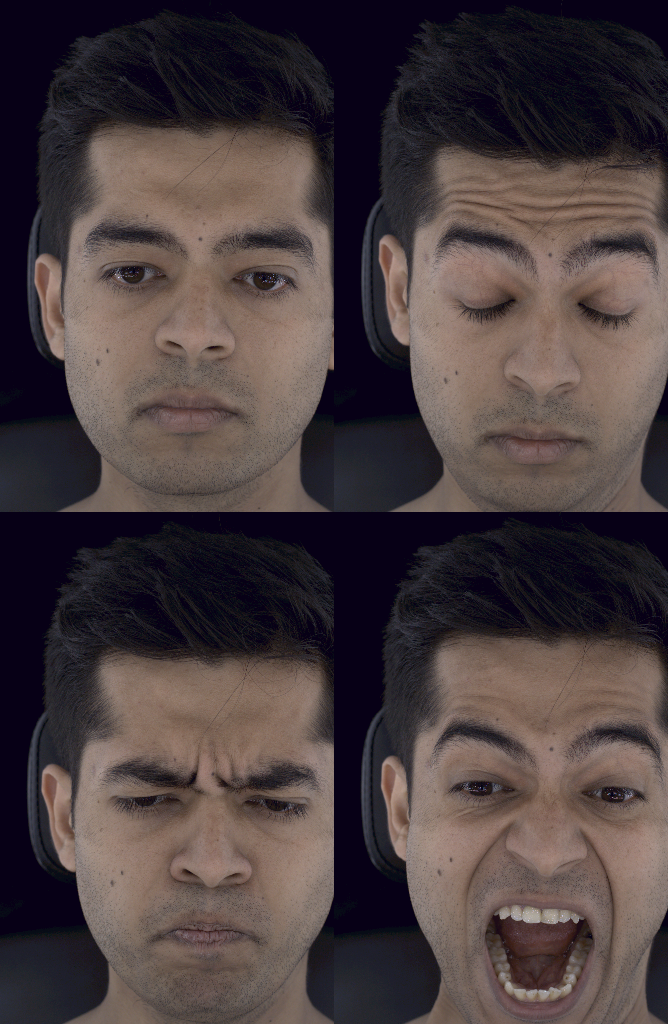
\includegraphics[width=\linewidth,trim={0 2em 0 2em}, clip]{assets/\blendfieldsdirname/rebuttal/frames.png}
  \caption{\textbf{Training frames} -- In~\cref{sec:blendfields-experiments}, we show results for the \blendfields trained on $\nExpr{=}5$ expressions.
    The images represent these expressions for one of the subjects.
    For each subject, we selected similar expressions to show all possible
    wrinkles when combined.
    Please note that we also include a ``neutral'' expression (the first from
    the left)---it is necessary to enable the learning of a face without any
    wrinkles.
    % model to learn 
  }
  \label{fig:blendfields-supplementary-training-frames}
\end{figure}
  \subsection{Training frames}
    We present in~\cref{fig:blendfields-supplementary-training-frames} example
    training frames for one of the subjects.
    Each frame is a multi-view frame captured with ${\approx} 35$ cameras (the
    number of available cameras varied slightly between subjects).

    \begin{table}[!t]
  \centering
  \resizebox{\linewidth}{!}{
    \begin{tabular}{lcccccc}
      \toprule
      \multirow{2}[2]{*}{Method}                         & \multicolumn{3}{c}{Casual Expressions} & \multicolumn{3}{c}{Novel Pose Synthesis}                                                                                                                                                  \\
      \cmidrule(lr){2-4}\cmidrule(lr){5-7}
                                                         & PSNR $\uparrow$                        & SSIM $\uparrow$                          & LPIPS $\downarrow$                & PSNR $\uparrow$                    & SSIM $\uparrow$                   & LPIPS $\downarrow$                \\
      \midrule
      NeRF \cite{mildenhall2020nerf}                     & 22.0060                                & 0.6556                                   & 0.3222                            & 23.8077                            & 0.7448                            & 0.2779                            \\
      Conditioned NeRF \cite{mildenhall2020nerf}         & 21.0846                                & 0.6280                                   & 0.3042                            & 22.9991                            & 0.7261                            & 0.2362                            \\
      NeRFies \cite{park2021nerfies}                     & 20.7004                                & 0.6076                                   & 0.3579                            & 23.0123                            & 0.7253                            & 0.2840                            \\
      HyperNeRF-AP \cite{park2021hypernerf}              & 20.8105                                & 0.6214                                   & 0.3504                            & 22.8193                            & 0.7185                            & 0.2689                            \\
      HyperNeRF-DS \cite{park2021hypernerf}              & 20.8847                                & 0.6111                                   & 0.3656                            & 23.0075                            & 0.7259                            & 0.2729                            \\
      \midrule
      VolTeMorph$_1$ \cite{garbin2024voltemorph}         & 21.3265                                & 0.7091                                   & 0.2706                            & 22.3007                            & 0.7795                            & \cellcolor{secondbestcolor}0.2281 \\
      VolTeMorph$_\text{avg}$\cite{garbin2022voltemorph} & \cellcolor{secondbestcolor}22.0759     & \cellcolor{secondbestcolor}0.7755        & \cellcolor{secondbestcolor}0.2615 & \cellcolor{secondbestcolor}23.8974 & \cellcolor{secondbestcolor}0.8458 & 0.2302                            \\
      \midrule
      \textbf{\methodname{}}                             & \cellcolor{firstbestcolor}22.8982      & \cellcolor{firstbestcolor}0.7954         & \cellcolor{firstbestcolor}0.2256  & \cellcolor{firstbestcolor}24.4432  & \cellcolor{firstbestcolor}0.8477  & \cellcolor{firstbestcolor}0.2052  \\
      \bottomrule
    \end{tabular}
  }
  \caption{\textbf{Quantitative results without masking} --
    Similarly to \cref{tab:blendfields-quantitative-results}, we compare \blendfields to other related approaches.
    However, we calculate the results over the whole image space, without
    removing the background.
    \blendfields and VolTeMorph~\cite{garbin2024voltemorph} model the background as a separate NeRF-based~\cite{mildenhall2020nerf} network.
    The points that do not fall into the tetrahedral mesh are assigned to the
    background.
    As the network overfits to sparse training views, it poorly extrapolates
    to novel expressions (as the new head pose or expression may reveal some
    unknown parts of the background) and views.
    At the same time, all other baselines do not have any mechanism to
    disambiguate the background and the foreground.
  }
  % }
  \label{tab:blendfields-quantitative-results-without-masking}
\end{table}
  \subsection{Quantitative results with background}
    We compare \blendfields and the baselines similarly
    to~\cref{subsec:blendfields-realistic-human-captures}.
    However, in this experiment, we deliberately include the background in
    metric calculation.
    We show the results in
    \cref{tab:blendfields-quantitative-results-without-masking}.
    In all the cases, \blendfields performs best even though the method was
    not designed to model the background accurately.
    Additionally, as HyperNeRF~\cite{park2021hypernerf},
    NeRFies~\cite{park2021nerfies}, and NeRF~\cite{mildenhall2020nerf} do not
    have any mechanism to disambiguate between the foreground and the
    background, the metrics are significantly worse when including the latter.

  \subsection{Additional qualitative results}

    We show in~\cref{fig:blendfields-qualitative-other-baselines} results of
    baselines that do not rely on parametric models of the
    face~\cite{li2017flame}.
    Compared to \blendfields, they cannot render high-fidelity faces.
    The issue comes from the assumed data sparsity---those approaches rely on
    the interpolation in the training data.
    As we assume access to just a few frames, there is no continuity in the
    training data that would guide them to interpolate between known
    expressions.
    \blendfields presents superior results given novel expressions even with such a sparse dataset.
    results.

    \clearpage
    
\renewcommand{\imagewidth}{3.3cm}
\renewcommand{\imageheight}{4.0263671874999996cm}
\renewcommand{\smallimagewidth}{0.8cm}
\renewcommand{\expressionsep}{0em}

\newcommand{\firstindex}{0189}
\newcommand{\secondindex}{0091}
\newcommand{\thirdindex}{0505}
\newcommand{\fourthindex}{0852}

\newcommand{\supimageoneindex}[2]{
  \includegraphics[width=\imagewidth, trim={0 0 0 0}, clip]{assets/\blendfieldsdirname/supplementary/expressions/#1_2183941_selected_rom_#2_\firstindex.png}
}
\newcommand{\supimagetwoindex}[2]{
  \includegraphics[width=\imagewidth, trim={0 0 0 0}, clip]{assets/\blendfieldsdirname/supplementary/expressions/#1_5372021_selected_rom_#2_\secondindex.png}
}
\newcommand{\supimagethreeindex}[2]{
  \includegraphics[width=\imagewidth, trim={0 0 0 0}, clip]{assets/\blendfieldsdirname/supplementary/expressions/#1_6795937_selected_rom_#2_\thirdindex.png}
}
\newcommand{\supimagefourindex}[2]{
  \includegraphics[width=\imagewidth, trim={0 0 0 0}, clip]{assets/\blendfieldsdirname/supplementary/expressions/#1_7889059_selected_rom_#2_\fourthindex.png}
}

\renewcommand{\versionone}{
  \begin{tikzpicture}[
      >=stealth',
      overlay/.style={
          anchor=south west,
          draw=black,
          rectangle,
          line width=0.8pt,
          outer sep=0,
          inner sep=0,
        },
    ]
    \matrix[
      matrix of nodes,
      column sep=0pt,
      row sep=0pt,
      ampersand replacement=\&,
      inner sep=0,
      outer sep=0,
      draw=black,
      rectangle,
      line width=0.5pt
    ] (gt) {
      \supimageoneindex{gt}{0}   \\
      \supimagetwoindex{gt}{0}   \\
      \supimagethreeindex{gt}{0} \\
      \supimagefourindex{gt}{0}  \\
    };

    \matrix[
      matrix of nodes,
      column sep=0pt,
      row sep=0pt,
      ampersand replacement=\&,
      inner sep=0,
      outer sep=0,
      right=0pt of gt-1-1.east,
      draw=black,
      rectangle,
      line width=0.5pt
    ] (k1) {
      \supimageoneindex{bv_aux}{0} \&
      \supimageoneindex{bv_aux}{0-1} \&
      \supimageoneindex{bv_aux}{0-1-2} \&
      \supimageoneindex{bv_aux}{0-1-2-3} \&
      \supimageoneindex{bv_aux}{0-1-2-3-4} \\
    };

    \matrix[
      matrix of nodes,
      column sep=0pt,
      row sep=0pt,
      ampersand replacement=\&,
      inner sep=0,
      outer sep=0,
      right=0pt of gt-2-1.east,
      draw=black,
      rectangle,
      line width=0.5pt
    ] (k2) {
      \supimagetwoindex{bv_aux}{0} \&
      \supimagetwoindex{bv_aux}{0-1} \&
      \supimagetwoindex{bv_aux}{0-1-2} \&
      \supimagetwoindex{bv_aux}{0-1-2-3} \&
      \supimagetwoindex{bv_aux}{0-1-2-3-4} \\
    };

    \matrix[
      matrix of nodes,
      column sep=0pt,
      row sep=0pt,
      ampersand replacement=\&,
      inner sep=0,
      outer sep=0,
      right=0pt of gt-3-1.east,
      draw=black,
      rectangle,
      line width=0.5pt
    ] (k3) {
      \supimagethreeindex{bv_aux}{0} \&
      \supimagethreeindex{bv_aux}{0-1} \&
      \supimagethreeindex{bv_aux}{0-1-2} \&
      \supimagethreeindex{bv_aux}{0-1-2-3} \&
      \supimagethreeindex{bv_aux}{0-1-2-3-4} \\
    };

    \matrix[
      matrix of nodes,
      column sep=0pt,
      row sep=0pt,
      ampersand replacement=\&,
      inner sep=0,
      outer sep=0,
      right=0pt of gt-4-1.east,
      draw=black,
      rectangle,
      line width=0.5pt
    ] (k4) {
      \supimagefourindex{bv_aux}{0} \&
      \supimagefourindex{bv_aux}{0-1} \&
      \supimagefourindex{bv_aux}{0-1-2} \&
      \supimagefourindex{bv_aux}{0-1-2-3} \&
      \supimagefourindex{bv_aux}{0-1-2-3-4} \\
    };

    \node[above=0em of gt-1-1.north, align=center, anchor=south]{Ground Truth};
    \node[above=0em of k1-1-1.north, align=center, anchor=south]{$K={1}$};
    \node[above=0em of k1-1-2.north, align=center, anchor=south]{$K={2}$};
    \node[above=0em of k1-1-3.north, align=center, anchor=south]{$K={3}$};
    \node[above=0em of k1-1-4.north, align=center, anchor=south]{$K={4}$};
    \node[above=0em of k1-1-5.north, align=center, anchor=south]{$K={5}$};

    \node[left=0em of gt-1-1.west, align=center, anchor=east]{\rotatebox{90}{\textsc{Subject} 2183941}};
    \node[above=0em of gt-2-1.west, align=center, anchor=east]{\rotatebox{90}{\textsc{Subject} 5372021}};
    \node[above=0em of gt-3-1.west, align=center, anchor=east]{\rotatebox{90}{\textsc{Subject} 6795937}};
    \node[above=0em of gt-4-1.west, align=center, anchor=east]{\rotatebox{90}{\textsc{Subject} 7889059}};
  \end{tikzpicture}
}

\begin{figure*}[htb]
  \centering
  \resizebox{\linewidth}{!}{
    \versionone
  }
  \caption{\textbf{Qualitative ablation over the number of training expressions} -- {
      We show qualitatively how the number of training expressions $\nExpr$
      affects the rendering quality.
      The first row shows the ground truth images.
      All other consecutive rows show the images rendered with \blendfields
      while increasing the number of training expressions.
      The last row, $\nExpr{=}5$ corresponds to the results presented in the
      main part of the article.
      The subject's naming follows the convention introduced in the Multiface
      repository~\cite{wuu2022multiface}.
      Please refer to~\cref{tab:blendfields-ablation-num-expressions-fix} for
      quantitative results.
    }}
  \label{fig:blendfields-qualitative-ablation-expressions}
\end{figure*}

    
\renewcommand{\imagewidth}{2.7cm}
\renewcommand{\imageheight}{4.0263671874999996cm}
\renewcommand{\smallimagewidth}{0.8cm}
\renewcommand{\expressionsep}{0em}

\renewcommand{\firstindex}{0580}
\renewcommand{\secondindex}{0378}
\renewcommand{\thirdindex}{0226}
\renewcommand{\fourthindex}{0720}

\renewcommand{\supimageoneindex}[1]{
  \includegraphics[width=\imagewidth, trim={0 0 0 0}, clip]{assets/\blendfieldsdirname/supplementary/baselines/#1_2183941_selected_rom_\firstindex.png}
}
\renewcommand{\supimagetwoindex}[1]{
  \includegraphics[width=\imagewidth, trim={0 0 0 0}, clip]{assets/\blendfieldsdirname/supplementary/baselines/#1_5372021_selected_rom_\secondindex.png}
}
\renewcommand{\supimagethreeindex}[1]{
  \includegraphics[width=\imagewidth, trim={0 0 0 0}, clip]{assets/\blendfieldsdirname/supplementary/baselines/#1_6795937_selected_rom_\thirdindex.png}
}
\renewcommand{\supimagefourindex}[1]{
  \includegraphics[width=\imagewidth, trim={0 0 0 0}, clip]{assets/\blendfieldsdirname/supplementary/baselines/#1_7889059_selected_rom_\fourthindex.png}
}

\renewcommand{\versionone}{
  \tikzsetnextfilename{blendfields_other_baselines}
  \begin{tikzpicture}[
      >=stealth',
      overlay/.style={
          anchor=south west,
          line width=0,
          outer sep=0,
          inner sep=0,
        },
    ]
    \matrix[
      matrix of nodes,
      column sep=0pt,
      row sep=0pt,
      ampersand replacement=\&,
      inner sep=0,
      outer sep=0,
      line width=0
    ] (gt) {
      \supimageoneindex{gt}   \\
      \supimagetwoindex{gt}   \\
      \supimagethreeindex{gt} \\
      \supimagefourindex{gt}  \\
    };

    \matrix[
      matrix of nodes,
      column sep=0pt,
      row sep=0pt,
      ampersand replacement=\&,
      inner sep=0,
      outer sep=0,
      right=0pt of gt-1-1.east,
      line width=0,
    ] (k1) {
      \supimageoneindex{bv_aux} \&
      \supimageoneindex{nerf}   \&
      \supimageoneindex{dnerf} \&
      \supimageoneindex{nerfies} \&
      \supimageoneindex{hypernerf_static}    \&
      \supimageoneindex{hypernerf_dynamic} \\
    };

    \matrix[
      matrix of nodes,
      column sep=0pt,
      row sep=0pt,
      ampersand replacement=\&,
      inner sep=0,
      outer sep=0,
      right=0pt of gt-2-1.east,
      line width=0,
    ] (k2) {
      \supimagetwoindex{bv_aux} \&
      \supimagetwoindex{nerf}   \&
      \supimagetwoindex{dnerf} \&
      \supimagetwoindex{nerfies} \&
      \supimagetwoindex{hypernerf_static}    \&
      \supimagetwoindex{hypernerf_dynamic} \\
    };

    \matrix[
      matrix of nodes,
      column sep=0pt,
      row sep=0pt,
      ampersand replacement=\&,
      inner sep=0,
      outer sep=0,
      right=0pt of gt-3-1.east,
      line width=0
    ] (k3) {
      \supimagethreeindex{bv_aux} \&
      \supimagethreeindex{nerf}   \&
      \supimagethreeindex{dnerf} \&
      \supimagethreeindex{nerfies} \&
      \supimagethreeindex{hypernerf_static}    \&
      \supimagethreeindex{hypernerf_dynamic} \\
    };

    \matrix[
      matrix of nodes,
      column sep=0pt,
      row sep=0pt,
      ampersand replacement=\&,
      inner sep=0,
      outer sep=0,
      right=0pt of gt-4-1.east,
      line width=0
    ] (k4) {
      \supimagefourindex{bv_aux} \&
      \supimagefourindex{nerf}   \&
      \supimagefourindex{dnerf} \&
      \supimagefourindex{nerfies} \&
      \supimagefourindex{hypernerf_static}    \&
      \supimagefourindex{hypernerf_dynamic} \\
    };

    \node[above=0em of gt-1-1.north, align=center, anchor=south]{Ground Truth};
    \node[above=0em of k1-1-1.north, align=center, anchor=south]{\textbf{\methodname{}}};
    \node[above=0em of k1-1-2.north, align=center, anchor=south]{NeRF};
    \node[above=0em of k1-1-3.north, align=center, anchor=south]{NeRF+expr};
    \node[above=0em of k1-1-4.north, align=center, anchor=south]{NeRFies};
    \node[above=0em of k1-1-5.north, align=center, anchor=south]{HyperNeRF-AP};
    \node[above=0em of k1-1-6.north, align=center, anchor=south]{HyperNeRF-DS};

    \node[left=0em of gt-1-1.west, align=center, anchor=east]{\rotatebox{90}{\textsc{Subject} 2183941}};
    \node[above=0em of gt-2-1.west, align=center, anchor=east]{\rotatebox{90}{\textsc{Subject} 5372021}};
    \node[above=0em of gt-3-1.west, align=center, anchor=east]{\rotatebox{90}{\textsc{Subject} 6795937}};
    \node[above=0em of gt-4-1.west, align=center, anchor=east]{\rotatebox{90}{\textsc{Subject} 7889059}};
  \end{tikzpicture}
}

\begin{figure*}[htb]
  \centering
  \resizebox{\linewidth}{!}{\versionone}
  \caption{\textbf{Comparison to strictly data-driven approaches} --
    We compare \blendfields to other baselines that do not rely on mesh-driven rendering: NeRF~\cite{mildenhall2020nerf}, NeRF conditioned on the expression code (NeRF+expr)~\cite{mildenhall2020nerf}, NeRFies~\cite{park2021nerfies}, and HyperNeRF-AP/DS~\cite{park2021hypernerf}.
    As a static model, NeRF converges to an average face from available
    ($\nExpr{=}5$) expressions.
    All other baselines exhibit severe artifacts compared to \blendfields.
    Those baselines rely on the data continuity in the training set (\eg, from
    a video), and cannot generalize to any other expression.
  }
  \label{fig:blendfields-qualitative-other-baselines}
\end{figure*}

